\documentclass[conference]{IEEEtran}
\IEEEoverridecommandlockouts
% The preceding line is only needed to identify funding in the first footnote. If that is unneeded, please comment it out.
\usepackage{cite}
\usepackage{amsmath,amssymb,amsfonts}
\usepackage{algorithmic}
\usepackage{graphicx}
\usepackage{textcomp}
\usepackage{xcolor}

\usepackage{multirow}
\usepackage{rotating}
\usepackage{tabularx,ragged2e,booktabs}
\usepackage{float}

\usepackage{svg}

\usepackage{mdframed}
\usepackage{hyperref}
\usepackage{tikz}
\usepackage{makecell}
\usepackage{tcolorbox}
\usepackage{amsthm}
%\usepackage[english]{babel}
\usepackage{pifont} % checkmarks
%\theoremstyle{definition}
%\newtheorem{definition}{Definition}[section]
\usepackage{fancyhdr}
\pagestyle{fancy}
\fancyhf{}
\fancyfoot[C]{\thepage}

\usepackage{listings}
\lstset
{ 
    basicstyle=\footnotesize,
    numbers=left,
    stepnumber=1,
    xleftmargin=5.0ex,
}


%SCJ
\usepackage{subcaption}
\usepackage{array, multirow}
\usepackage{enumitem}




\def\BibTeX{{\rm B\kern-.05em{\sc i\kern-.025em b}\kern-.08em
    T\kern-.1667em\lower.7ex\hbox{E}\kern-.125emX}}
\begin{document}

%\IEEEpubid{978-1-6654-8356-8/22/\$31.00 ©2022 IEEE}
% @Sune:
% Found this suggestion: https://site.ieee.org/compel2018/ieee-copyright-notice/
% I have added it - you can see if it fulfills the requirements

%\IEEEoverridecommandlockouts
%\IEEEpubid{\makebox[\columnwidth]{978-1-6654-8356-8/22/\$31.00 ©2022 IEEE %\hfill} \hspace{\columnsep}\makebox[\columnwidth]{ }}
%978-1-6654-8356-8/22/$31.00 ©2022 IEEE
% copyright notice added:
%\makeatletter
%\setlength{\footskip}{20pt} 
%\def\ps@IEEEtitlepagestyle{%
%  \def\@oddfoot{\mycopyrightnotice}%
%  \def\@evenfoot{}%
%}
%\def\mycopyrightnotice{%
%  {\footnotesize 978-1-6654-8356-8/22/\$31.00 ©2022 IEEE\hfill}% <--- Change here
%  \gdef\mycopyrightnotice{}% just in case
%}


\title{Group Report Template\\
}

\author{
    \IEEEauthorblockN{
        Stefan-Daniel Horvath\IEEEauthorrefmark{1},
        Michael H Pedersen\IEEEauthorrefmark{1},
        Jacob B Florczak\IEEEauthorrefmark{1},
        Ignatios Mantanis\IEEEauthorrefmark{1},
    }
    \IEEEauthorblockA{
        University of Southern Denmark, SDU Software Engineering, Odense, Denmark \\
        Email: \IEEEauthorrefmark{1} \textnormal{\{sthor23,micpe18,jaflo18,igman23\}}@student.sdu.dk
    }
}


%%%%

%\author{\IEEEauthorblockN{1\textsuperscript{st} Blinded for review}
%\IEEEauthorblockA{\textit{Blinded for review} \\
%\textit{Blinded for review}\\
%Blinded for review \\
%Blinded for review}
%\and
%\IEEEauthorblockN{2\textsuperscript{nd} Blinded for review}
%\IEEEauthorblockA{\textit{Blinded for review} \\
%\textit{Blinded for review}\\
%Blinded for review \\
%Blinded for review}
%\and
%\IEEEauthorblockN{3\textsuperscript{nd} Blinded for review}
%\IEEEauthorblockA{\textit{Blinded for review} \\
%\textit{Blinded for review}\\
%Blinded for review \\
%Blinded for review}
%}

%%%%
%\IEEEauthorblockN{2\textsuperscript{nd} Given Name Surname}
%\IEEEauthorblockA{\textit{dept. name of organization (of Aff.)} \\
%\textit{name of organization (of Aff.)}\\
%City, Country \\
%email address or ORCID}



\maketitle
\IEEEpubidadjcol
\begin{abstract}
    %%%%%%%%%%%%%%%%%% Max 970 signs without space %%%%%%%%%%%%%%%%%%
    % Intro

    % Gab

    % Aim 

    % Method

    % Results 

    The following paper presents the results that were achieved by the group in the course Advanced topics in software architecture at the University of Southern Denmark. The focus of the project was to design a software architecture in the conext of Industry 4.0 and smart farming with a focus on livestock farming. Within the domain of smart farming for livestock there has for many years been a lack of adoption for Industry 4.0 concepts. The goal for the project were then to identify the challenges that are present in the domain and design and develop a prtotype that incorporates industry 4.0 concepts and showcases how such a system might look like. The system is evaluated based on different qualit attributes and quality attribute scenarios. The results of the evaluation shows that the system is able to adhere to the defined quality attributes and quality attribute scenarios.
\end{abstract}

\begin{IEEEkeywords}
    Smart farming, Industry 4.0, Keyword3, Keyword4, Keyword5
\end{IEEEkeywords}

\section{Introduction and Motivation}
%Introduction and motivate the problem
The advancement of technology is at an all-time high and the possibilities using technology are expanding rapidly. Several industries are benefitting using assembly robots, self-driving forklifts, etc. People, machines, and products are directly related to each other. The term "Industry 4.0" describes \textit{the intelligent networking of machines and processes for industry with the help of information and communication technology} \cite{plattformindustrie40}. The principles of Industry 4.0 result in several benefits, including the possibility of flexibility within production, ability to quickly change a production line for a different task, and many more \cite{plattformindustrie40}. \vspace{2mm} \newline
This concept introduces the need for many different systems to be able to communicate in one way or another, which is one of the big challenges Industry 4.0 is faced with \cite{PANETTO2019198}. Therefore, for a system to successfully adhere to Industry 4.0 principles it must be capable of communicating between subsystems and various types of hardware within the system. \newline
Industry 4.0 might originally have been coind for the manufacturing industry, but the potential of the concept is not limited to this industry alone. There is great potential for farming to adapt to the principles also. By incorporating the power of real-time data, IoT (internet of things) and analytics, farmers can respond to more nuanced changes in the environnment and the health of the animals. This not only has great benefits for the productivity of the farm, but also has benefits for a more sustainable farming industry. \newline
In this paper the intent of the project is to create a system that can handle various aspects of production, including monitoring biometrics, managing feed, and handling orders in a fully automated livestock farming system. \vspace{2mm} \newline
\textit{Therefore this paper designs and implements an architecture based on a smart livestock farming system. The system is evaluated by its ability to adhere to stated quality attributes}.
The motivation behind designing such a system is based on the need for interoperability between different systems, which in its current state in farming is one of the major challenges. The lack of communication between these technologies hampers their synergistic use by farmers \cite{app122412844}. Through our work, we aim to address these challenges and contribute to the seamless integration of diverse technologies. \vspace{3mm}






The structure of the paper is as follows.
Section \ref{sec:problem} outlines the research question and the research approach.
%to analyze the research question and evaluate our results.
Section \ref{sec:related_work} describes similar work in the field and how our contribution fits the field.
Section \ref{sec:use_case} presents a use case of the system, which gives us a better representation of what the system is able to do.
The use case serves as input to specify QA requirements for the system \ref{sec:qas}.
Section \ref{sec:middleware_architecture} introduces the proposed software architecture design for the system.
Section \ref{sec:evaluation} evaluates the proposed architecture on tests conducted on the system and analyzes the results against the stated QA requirement.


\section{Problem and Approach}
% conext:
% This is a secitoin talking about the problem that we are facing in this ?project. The project is about Indystry 4.0 in a livestock farm setting.
% we have differnet services and serves in a Java-based agricultural management system for cattle farming that integrates several services: an Outbound Department for order management, a Laboratory/QA for product testing and compliance monitoring, and a Farmer GUI for user interactions. It employs a Message Bus for inter-service communication and Bio-monitoring for livestock health tracking, utilizing both MySQL and semi-structured databases. An Inbound service manages stock and orders, while the Feed System oversees feed conditions and inventory. The system is sensor-reliant, with various sensors providing real-time data on cattle health, environmental conditions, and feed storage, interfacing with a Hadoop big data server for analytics and reporting.

\label{sec:problem}
\emph{Problem.}
In livestock farming, the production process is highly dependent on the environment and the health of the animals. To address this the system that has been developed in this project aims to look into how differnet arcitectural approaches can bridge differnet services and servers in a way that the production process can be reconfigured to adapt to the changes in the environment and the health of the animals. To approach this problem the following research questions are formulated:

\emph{Research questions:}
\begin{enumerate}
    
\end{enumerate}


\emph{Approach.}
The following steps are taken to answer this paper's research questions: 
\begin{enumerate}
    \item 
\end{enumerate}


\section{Related work}
\label{sec:related_work}
This section addresses existing knowledge and contributions by examining Industry 4.0 and its current use within the livestock and agricultural domain. In total, eight papers are investigated using a systematic literature review. \vspace{2mm}
\newline
Over the past years, large parts of the industry have been undergoing the revolution to Industry 4.0, integrating higher levels of technology into the lifecycle of products. Order systems, production environments and shipment as well as maintenance of products became more automated and integrated different, interconnected smart systems.
However, the primary sector, mainly the agricultural part of industry, has not kept up with the rapid changes to modern production standards \cite{pr7010036}.
This project plan to design an Industry 4.0 architecture for a prototype system for the livestock farming domain. For that, the project begins with evaluating which needs and challenges are already reported on for similar systems in the domain and find existing suggestions for designing such systems.
In detail, a small but concise systematic literature review is performed considering the following research questions:
\vspace{2mm}
\begin{itemize}
    \item What functional requirements are considered important for agricultural industry 4.0 systems in existing literature?
    \item Do suggestions for parts of the architecture and technologies of systems exist that support the requirements of agricultural industry 4.0 systems?
    \item What are current challenges within agricultural industry 4.0 systems in use?
\end{itemize}
\vspace{2mm}

To answer these questions, an examination of the scientific reports ragarding Industry 4.0 concepts and software in the livestock farming and agricultural context is conducted. For the process of identifying appropriate research, a semi-automated search strategy as well as snowball techniques after finding promising starting point papers. This search is conducted across a spectrum of academic digital databases, including MPBI, ProQuest, DOAJ, Google Scholar, and ScienceDirect. A set of inclusion criteria was utilized with the purpose of gathering appropriate articles, reviews and case studies published in English within a timeline of the last 7 years. This approach is designed to collate a comprehensive and current body of knowledge, providing a solid foundation for the study.
\vspace{2mm}
\\
The keyword search focused on a list of keywords and key phrases related to the research questions. That list included the words Industry 4.0, agriculture, agriculture 4.0, farming, livestock, and any related phrases. Evaluating the search results, the ones which were applicable to the above-mentioned criteria and related to the research questions and challenges were chosen (excluding some papers with a focus on machine learning, since they were not related to the architectural parts of software design).
Additionally, ensuring that the papers present a balanced view by considering various perspectives and supporting their arguments with evidence from diverse sources, such as references and/or observed data was important. It was also checked that the authors have taken care to present the information objectively, avoiding bias in their analysis.
\vspace{2mm}
\newline
To report similar or different aspects covered in the different papers, it was determined three categories covered in most of the papers. These categories are “Functional requirements and quality attributes”, “Architectural aspects” and “Existing challenges/problems”. For each of them, an overview of the most important points made is given below.
\newline
\subsection{Functional requirements and quality attributes}
The most common quality attribute for agriculture 4.0 systems throughout the list of papers is interoperability of different subsystems. All the listed papers either mention this attribute directly or refer to middleware products, which are the heart of interoperability between different subsystems.
Similarly, flexibility of the system, for example being able to add new subsystems or change parts of the software, is addressed as an important attribute in several papers \cite{KRUIZE201612}, \cite{app122412844}, \cite{jepsen2021analysis}, \cite{10092655}.
Another common attribute is scalability, which papers \cite{KRUIZE201612}, \cite{agronomy12030750}, \cite{s22124319} directly address. In the context of a farm there is a possibility of it growing over time, it is therefore important that the system capable of scaling and can adapt to larger amounts of data and the added workload.
A few of the papers \cite{agronomy12030750}, \cite{s22124319} also mentions security as an important attribute of large-scale systems, so that the data and system can't be tampered with.
While there were little contradicting opinions on attributes, different papers had different focus points. A few attributes worth mentioning include component availability \cite{KRUIZE201612}, reconfigurability \cite{10092655} or accuracy of systems \cite{ZHANG2021127712}.
\newline
\subsection{Architectural aspects}
Several of the papers formulate guidelines or opinions on different architectural aspects of agricultural 4.0 systems. To address the above mentioned interoperability requirement, most papers \cite{KRUIZE201612}, \cite{app122412844}, \cite{agronomy12030750}, \cite{jepsen2021analysis}, \cite{10092655}, \cite{ZHANG2021127712} directly focus on middleware components that are used to orchestrate and abstract between different subsystems. In this context, they also mention well-defined interfaces for the communication between different components.
Another directly addressed aspect is the virtualization \cite{pr7010036}, \cite{KRUIZE201612} of different components in the actual physical farm, so that they can be included in the software ecosystem.
While different explicit technologies are addressed by different papers (Docker, Kafka, etc.), a more abstract technological term across different papers is “IoT” \cite{pr7010036}, \cite{agronomy12030750}, \cite{s22124319}, \cite{ZHANG2021127712}. Since many systems in the agricultural context rely on sensor data and physical devices (robots, vehicles), the inclusion of IoT devices is necessary for agriculture 4.0 systems.
\newline
\subsection{Existing challenges/problems}
Several of the papers \cite{pr7010036}, \cite{KRUIZE201612}, \cite{app122412844}, \cite{agronomy12030750}, \cite{s22124319}, \cite{jepsen2021analysis}, \cite{ZHANG2021127712} come to the conclusion that many technologies exist that try to make livestock farming smarter and more efficient, but the problem with the technologies is that often coordination problems occur making the interoperability difficult to achieve. A gap in this is the need for common communication protocols or orchestration middleware that these technologies can share so data can be used for shared interests.
Additional reported challenges exist within the integration of 4.0 systems to the actual farms, which include high financial costs and missing expertise for technological equipment and systems \cite{app122412844}, \cite{s22124319}, \cite{ZHANG2021127712}. To counteract some of these issues, there could be governmental policies, which are at this point still undeveloped \cite{pr7010036}.
Another reported issue might be bandwidth problems in rural areas, which would restrict large interconnected systems with many components \cite{pr7010036}, \cite{s22124319}.
\newline

All contributions provide valuable knowledge about Industry 4.0 and its usage within modern agriculture and livestock farming. However, a notable gap in existing literature is the absence of real-world examples of successful or unsuccessful implementations of livestock farming systems that apply Industry 4.0 principles. Developing practical examples can help provide a clearer understanding of how to solve the challenges of Industry 4.0 within the livestock farming domain.

\section{Use Case and Quality Attribute Scenario}
\label{sec:use_case_and_qas}
This Section introduces the use cases and the specified QASes.
The QASes are developed based on the use cases.

\subsection{Use cases}
\label{sec:use_case}
To better grasp the ability of the system, several use cases have been constructed. The use cases assists to identify systems and subsystems needed to implement the system.
Its important to also consider the quality of the system that goes beyond just functionality. This will be refered to as quality attributes \cite{bass2021software}. \vspace{2mm}

\subsubsection{Automatic feed ordering}
\label{sec:use_case_feed}
The first use case outlines an automatic order placement for more feed, which is triggered by low feed stock levels. This use case contains three actors: A feed distributor, a control system and a feed vendor.
Events in this use case is the feed distributor continously monitors feed levels and when the stock reaches below a certain amount it triggers a signal which gets sent to the control system.
The control system recieves the signal and creates the order for more feed, which it then forwards to the vendor system.
The vendor recieves order and checks for availability of feed for the incoming order. In case of resource shortage the vendor notifies the control system, so that the farmer can take action accordingly.
If resource are available the vendor schedules packaging of the feed and makes sure it is shipped to the farm and the control panel is notified of the order completion. From the time that the feed distributor recieves a signal of low stock the whole sequence must be finished within a resonable timeframe. \vspace{2mm} \newline
From this use case it is possible to derive several systems already for the management of livestock feed. First off for the feed distributor to know how much feed is currently in the silo on the farm, it needs information on the current stock. This could be done with a weight sensor in the silo but implmentations could varie. The feed distributor is then designed to act upon the stock of the silo reaches below a certain point. \vspace{2mm} \newline
The use case also describes a control system which handles the signal from the feed distributor and the creation of the order for the vendor, the vendor in this case is an external system that is not included in the prototybe system.

\subsubsection{Detect changes in livestock conditions}
This use case describes a scenario that can alert the farmer of the wellbeings of the livestock. This use case contains four actors: Sensors, a health analyzer, a control system and the farmer.
Eevnts in this use case is first of initiated by continously data being generated by sensors that are either attached to the livestock or its surroundings. This data is being transmitted into a storage system which then can be used to analyze the health of the livestock.
The health analyzer will then analyze the sensor data and if the data suggests e.g. a disease or other forms of the livestocks condition being worsened the system will transmit a warning to the control panel.
The control panel can be accessed by the farmer and the alert from the health analyzer will be able to tell the farmer which actions are required. The system should be able to handle the addition of new livestock, this will result in more sensors being added which should be completed with no downtime of the system.
In case of added load by the addition of more sensors, the system should be able to handle the increased load by dynamically scaling the storage. \vspace{2mm} \newline
From this use case more systems was identified to be implemented in the system. The control panel is already mentioned from the previous use case.
A system for the sensors are needed to transmit the data in to some form of storage system. The sensors will be generating a great amount of data, so the system should be able to handle a high throughput of data and also store a large amount of it.
This storage system can then be accessed by the health analyzer, which should be able to able to alert the farmer and also inform of the necessary actions. \newline

\subsection{Quality attribute scenarios}
\label{sec:qas}
To define success criteria for the system, several quality attribute scenarios have been created. These are used for setting up a scenario in which one of the quality attributes of the system gets addressed \cite{bass2021software}. This is helpful for testing the capabilities of the system.
A template for defining QASes is used for the creation of these scenarios. The templates captures a scenario through \textit{Source, Stimulus, Artifact, Environment, Response and Response measure} to which the requirement should apply \cite{bass2021software}. \newline
For the system in this paper there is specified three main requirements:
\begin{enumerate}
    \item Production software must be able to exchange and coordinate information to execut a prodcution and change production.
    \item Production software must run 24/7
    \item Production software must be continously deployable
\end{enumerate}
These three requirements can be directly translated to quality attributes. The first one refers to interoperability, the second availability and the third is described by deployability. \newline

\subsubsection{Interoperability}

\begin{table}[h]
    \renewcommand{\arraystretch}{1.3}
    \caption{Interoperability quality attribute scenarios}
    \label{interoperability}
    \centering
    \begin{tabularx}{\columnwidth}{>{\hsize=0.3\hsize}X>{\hsize=0.7\hsize}X}
        \hline
        \textbf{Portion of scenario} & \textbf{Value}                                                                               \\
        \hline
        Source                       & Feed distributor system.                                                                     \\
        Stimulus                     & A signal from the feed distributor indicating low feed stock.                                \\
        Artifact                     & Control system.                                                                              \\
        Environment                  & Normal operation during low feed stock.                                                      \\
        Response                     & The control system successfully creates and forwards an order to the external vendor system. \\
        Response measure             & The order is accuratly transmitted and the external vendor acknowledges it wihtin 5 seconds. \\
        \hline
    \end{tabularx}
\end{table}

Table \ref{interoperability} is a scenario for the interoperability quality attribute, which referes to the ability of two or more systems to be able to exchange and use information \cite{brownsword_2004}.
For the interoperability QAS, the scenario described is the ability of the system to be able to react to low feed stock and therefore make sure the necessary communication is carried out with other systems, this includes both the external vendor but also the control system.
The \textit{Source} in this scenario is the feed distributor system, which triggers the \textit{Stimulus}, in this case the indication of low feed stock. The stimulus arrives at the \textit{Artifact} (the control system), which is responsible for creating the order for feed. The \textit{Environment} assumes the condition of the component / system, which in this case is assumed to be under normal operation.
The \textit{Response} describes a process that handles the stimulus, so the system should be able to successfully create and forward the order. To be able to determine if the requirement from the scenario is satisfied the \textit{Response measure} is specified, which in this scenario specifies that the whole process should be transmitted and acknowledged within a certain timeframe (in this case 5 seconds). \newline

\subsubsection{Availability}

\begin{table}[h]
    \renewcommand{\arraystretch}{1.3}
    \caption{Availability quality attribute scenarios}
    \label{availability}
    \centering
    \begin{tabularx}{\columnwidth}{>{\hsize=0.3\hsize}X>{\hsize=0.7\hsize}X}
        \hline
        \textbf{Portion of scenario} & \textbf{Value}                                                                                           \\
        \hline
        Source                       & High sensor data throughput.                                                                             \\
        Stimulus                     & The message bus experiences an overload, causing the loss of a partition.                                \\
        Artifact                     & Message bus.                                                                                             \\
        Environment                  & Overloaded condition.                                                                                    \\
        Response                     & Due to the replication factor, the system ensures that the lost partition's data is still available.     \\
        Response measure             & The system maintains data integrity and availability through replication, even when a partition is lost. \\
        \hline
    \end{tabularx}
\end{table}

Table \ref{availability} is a scenario for the availability quality attribute, which refers to the systems ability to be ready to carry out a task, but it also covers the systems ability to mask or repair faults \cite{bass2021software}.
For the availability QAS, the scenario described is the systems ability to handle added load from the throughput of sensor data. The system should from the added load be able to circumvent the loss of data or the system becoming degraded in performance.
The \textit{Source} is coming from the sensor data throughput, which as described by the \textit{Stimulus} causes loss of a partition within the \textit{Artifact} (the message bus). The \textit{Environment} is assumed to be in an overloaded condition due to the amount of data causing the loss of a partition in the message bus.
The \textit{Response} handles the stimulus by applyin tactics or patterns to address the availability of the system in the case of a partition loss. The \textit{Response measure} indicates the handling of the fault should result in no data lost and the system to be with no downtime. \newline
\subsubsection{Deployability}

\begin{table}[h]
    \renewcommand{\arraystretch}{1.3}
    \caption{Deployability quality attribute scenarios}
    \label{deployability}
    \centering
    \begin{tabularx}{\columnwidth}{>{\hsize=0.3\hsize}X>{\hsize=0.7\hsize}X}
        \hline
        \textbf{Portion of scenario} & \textbf{Value}                                                                                                        \\
        \hline
        Source                       & Increased livestock population.                                                                                       \\
        Stimulus                     & Addition of more sensors to the livestock monitoring system.                                                          \\
        Artifact                     & Sensor system.                                                                                                        \\
        Environment                  & Deployment of additional sensors.                                                                                     \\
        Response                     & The system allows plug-and-play functionality, allowing quick and straight forward integration of additional sensors. \\
        Response measure             & New sensors can be deployed and be operational without downtime or configuration challenges.                          \\
        \hline
    \end{tabularx}
\end{table}


Table \ref{deployability} presents a scenario for the deployability of the system. Deployability refers to the system's ability to be updated continuously without requiring downtime, as described in \cite{bass2021software}. The goal is to expedite integration, enabling the development team to rapidly deploy updates to the production system.
For the deployability QAS, the scenario described highlights the systems ability to increase the amount sensors in the system. The system should be able to handle the added sensors without the need for downtime in the system.
The \textit{Source} is the increased livestock population which triggers the \textit{Stimulus} which is the addition of sensors. This is handled within the \textit{Artifact} (the sensor system), and the \textit{Environment} is the deployment of the additional sensors.
The \textit{Response} describes the systems ability to allow plug-and-play functionality, which allows for quick and easy integration of additional sensors. The \textit{Response measure} implies the process should be completed with no system downtime and configuration challenges. \newline


\section{The solution}
\label{sec:middleware_architecture}

% Description of the overall architecture designs
% Argue for tactics used to archieve the QASes
% Discuss the trade-offs
This section outlines the proposed technological solution for the medium-sized cattle farm. The design integrates various hardware and software components such as sensors, Java-based subsystems, message bus for middleware communication and Big data server for storing data. The whole purpose of this solution is to address the unique needs of the farm's operations which include animal care, feed management, and sales.

\subsection{\textbf{System Overview}}
The proposed system integrates biometric and feed monitoring, automated feeding, and resource management, ensuring efficiency and sustainability in farm operations. It is designed to manage around 100 animals, utilizing 200 to 300 sensors for various monitoring purposes such as monitoring the heart rate of cows, temperature or humidity of silos. In order for the system to be successful, continuous interoperability among various departments and their Java-based subsystems need to exist. Therefore, a robust middleware communication system facilitated by a central message bus was chosen to be used as the optimal architecture. \newline
\begin{figure*}[!ht]
    \centering
    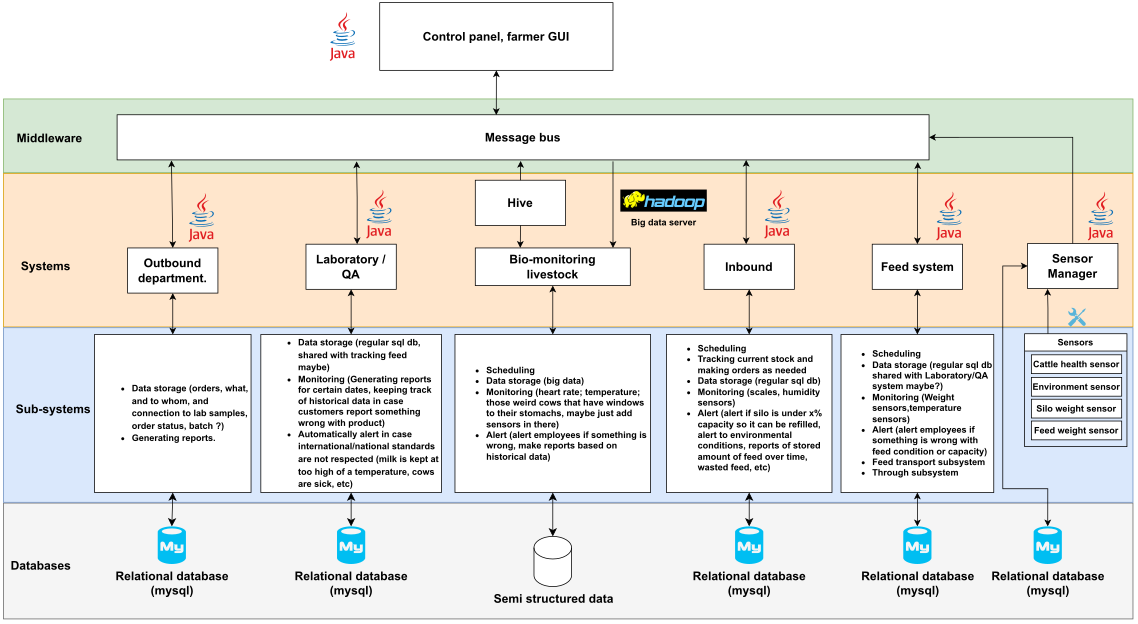
\includegraphics[width=\textwidth]{Images/architecture.pdf}
    \caption{The proposed architecture}
    \label{fig:systemArch}
\end{figure*}

Figure \ref{fig:systemArch} depicts the initial architecture that was drafted for the system. A few of these systems are not present in the final system implementation, but there will be enough implementation to show how the system adheres to the required quality attributes which are specified in the quality attribute scenarios from section \ref{sec:qas} and how the rest of the system can be implemented.
\subsection{\textbf{Middleware and Communication}}
For an Industry 4.0 system the middleware is the center of attention. From related work knowledge was obtained that highlighted the need for interoperability between different systems, this is where the message bus comes into play. \vspace{2mm} \\
Apache Kafka \cite{Apache2022Connect} has been selected for real-time data handling and as a central component of the message bus due to its distinct advantages in large-scale applications. Kafka offers high throughput and low latency, making it ideal for managing huge streams of sensor data in real-time. Furthermore, Kafka's ecosystem, including Kafka Connect, enables the efficient processing of big data, an essential requirement for the project. \vspace{2mm} \\

The distributed nature of Kafka uses multiple brokers, which for Kafka means that it has several servers to recieve and send data. This helps avoid a single point of failure and ensures system reliability. Kafka uses multiple tactics to achieve it's fault tolerance, one being replication of data across multiple brokers, which ensures if a broker is lost no data will be lost \cite{AltexSoft_2022}. This behavior is needed for the QAS described for availability in the system.
Besides affecting the QAS, Kafka also has great support for a variety of different systems and languages \cite{AltexSoft_2022}, which will support the interoperability of the system. \vspace{2mm}

The main downsides of using Kafka is the technological complexity and lack of management and monitoring tools. This presents a challenge and necessitates additional effort in system administration. Despite these challenges, Kafka's performance, scalability, and the ability to integrate with various technologies such as Hadoop for big data needs, make it the most suitable choice for the system. \vspace{2mm}


\subsection{\textbf{Subsystem Integration}}
Each department's Java-based subsystem operates through the middleware message bus, carrying out specific functions that are essential for each department needs. \vspace{2mm}\\
The choice of using Java-based subsystems can be described by several factors. Firstly, Java is an object-oriented programming language which makes for easier implementation as it allows for breaking the code into smaller, more manageable parts. \cite{Team_2022}.
Another important feature of Java is the ability to run on many devices, with different operating systems and hardware configurations. The interoperability of Java is what allows us to develop with a wide variety of systems. It supports \textit{deployability} by being platform independent and having standardized packaging. \vspace{2mm} \\
Java also provides automatic garbage collection, which helps it manage memory efficiently \cite{Team_2022}. This supports the \textit{availability} of the system by reducing the likelihood of memory errors.
Even though Java supports some of the system requirements, it also has tradeoffs. Just as automatic garbage collection is a plus, it also affects performance by always running in the background, where in languages like C or C++ this does not happen \cite{Team_2022}. \vspace{1mm}

\subsection{\textbf{Sensor Implementation}}
The farm’s operations are monitored by an array of sensors that perform various functions. Cattle health sensors monitor vital signs such as heart rate and body temperature, providing critical data for early illness detection. Environmental sensors monitor conditions on the farm, including temperature and humidity levels within the fields, the barns and silos. Silo weight sensors monitor and measures the amount of feed stored, and feed weight sensors keep track of distribution of feed to the cattle farm. \vspace{2mm} \\
All sensors are connected to a central middleware message bus, which uses Kafka to stream sensor data. This design allows the data to be analyzed and ingested into Hadoop Distributed file system (abriviated HDFS for later reference), from where it can be queried and used in reports. Kafka’s distributed nature and streaming capabilities enable the system to handle the influx of data from potentially hundreds of sensors without loss of information or delay, ensuring that the most current data is always available for decision-making processes. \vspace{2mm}

\subsection{\textbf{Database Management}}
A relational database using MySQL is employed across the Java-based subsystems, providing a consistent framework for data management.
The use of MySQL which is a relational database makes sense for the most of the subsystems in the architecture, because here it is not necessary to store live data but more historical data. MySQL also supports some of the quality attributes for the system. Just like Java, MySQL is platform independent \cite{Blue}, which means it supports \textit{deployability} by requiring no modification regardless of where it is running.
The main disadvantage of MySQL is the poor performance when exposed to high loads \cite{Blue}. Looking at the specified architecture there is  another system for storing the sensor data, which will handle the larger amounts of data better.

\subsection{\textbf{Bio-monitoring Livestock System}}
\subsubsection{Hardware}
Sensors are attached to each animal for monitoring temperature and heart rate, ensuring 24/7 health surveillance.\vspace{2mm}
\subsubsection{Software}
A Big Data architecture is employed, leveraging Kafka for robust data ingestion into HDFS. Kafka serves as a high-throughput distributed messaging system, capable of handling the streams of sensor data in real-time. It is chosen for its fault tolerance, durability, and ability to process data streams as continuous flows, which is critical for timely and accurate monitoring of livestock health.\vspace{2mm}
\subsubsection{Functionality}
The system operates continuously, utilizing Machine Learning to analyze the data and detect early signs of illness, notifying in time the animal care department. Kafka's immediate and efficient processing of data ensures speed and time efficiency to the system.\vspace{2mm}


\subsection{\textbf{Feed System}}
\subsubsection{Hardware}
Automated feeders equipped with sensors to control and monitor feed distribution.\vspace{2mm}
\subsubsection{Software}
Java-based control system to manage feeding operations, ensuring consistent and accurate feeding.\vspace{2mm}
\subsubsection{Functionality}
Real-time 24/7 monitoring with error detection and alerting mechanisms for immediate handling of issues.

\subsection{\textbf{Inbound System}}
\subsubsection{Hardware}
Feed silos equipped with scales and humidity sensors.\vspace{2mm}
\subsubsection{Software}
Java and MySQL manage data capturing and processing, facilitating efficient feed utilization and ordering.\vspace{2mm}
\subsubsection{Functionality}
Regular monitoring and data capture optimize feed management and resource planning.

\subsection{\textbf{Outbound System}}
Developed in Java, this MVC application manages customer orders, linking them with laboratory samples for efficient tracking and processing.

\subsection{\textbf{Hardware and Software Synergy}}
The sensor data is being mimicked by a Java application, that can simulate live sensor data. This allows for the posibility of evaluating on the systems capabilities in regards to data throughput.

\subsection{\textbf{Integration with HFDS}}
The integration of Kafka with the HDFS is a necessary decision to manage the large volumes of data generated by the biometric and environmental sensors. HDFS provides a reliable and scalable storage solution, capable of handling vast amounts of data while ensuring data integrity and accessibility. This integration allows for efficient data processing, storage, and retrieval, which are crucial for the real-time monitoring and analysis required in the bio-monitoring livestock system. \vspace{2mm} \\
HDFS supports several of the quality attributes required by the system. The main reasoning behind the use of it is because of the limited storage possibilites by MySQL, in HDFS it is possible to store extremely large amounts of data.
HDFS enhances the \textit{availability} by implementation of fault tolerance. As Kafka can replicate the data, same goes for HDFS, which means that it replicates the data across several nodes (physical computers) in a cluster (a group of physical computers) \cite{AltexSoft_2022a}. When a node fails no data is therefore lost, this refers to the tactic \textit{voting} which defines replication as a way of detecting faults \cite{Bass2012Software}.
HDFS is also able to scale horizontally which allows for a simple way to add more capacity for storing data. HDFS is located within the Apache ecosystem which provides a handful of different technologies for different use cases \cite{AltexSoft_2022a}, this improves the interoperability of the system as HDFS is able to communicate with various different technologies. As for the deployability of HDFS it is built on Java, which as mentioned can run on any system or hardware.\vspace{2mm} \\
When using HDFS it is important to consider that the files that are being stored are not too small. This is a disadvantages of HDFS, it has very poor handling of small files, in which case it is better to use SQL.
HDFS also has its own processing when trying to read data called MapReduce, which can be very slow and resource intensive when trying to process big data. Using Apache Hive can help aleviate this issue. Apache Hive is a data warehousing solution built on top of Apache Hadoop. It is designed to manage and query large datasets residing in distributed storage using a SQL-like syntax. Hive is particularly useful in systems that involve processing and analyzing big data, such as the sensor data in our project \cite{ApacheHive}.
The one downside that is provided by Hive is it doesnt handle real-time data querying, so in this system Hive would be used for looking at historical data \cite{ApacheHive}. Therefore the need for live data from the sensors is obtained from an intermediate data storage in the message bus (Kafka).

\subsection{\textbf{Containerization using Docker}}
For running the system it was containerized using Docker. Docker is a piece software that allows an open platform for developing, shipping and running applications \cite{Docker2022What}. It packages up code and its dependencies, which ensures that the applications run quickly and reliably from one environment to another \cite{Docker2022What}.
For the architecture proposed in the solution, each system has its own container and with all the systems containerized, it is possible to perform tests on the system using a single machine.\vspace{2mm} \\ Containerization helps isolate each system and therefore reducing conflicts between systems. Docker makes use of a few tactics to adhere to these principles that are connected to the \textit{deployability} QA. For managing the deployment pipeline it makes use of the \textit{Script deployment command} tactic which describes a script can do all the steps necessary for executing the deployment of the system as a whole \cite{Bass2012Software}. For managing the deployed system it also makes use of the \textit{Pacakge dependencies} which essentially describes how it packages the system, that leads to containerization \cite{Bass2012Software}.


\subsection{\textbf{Discussion on Trade-offs}}
The selection of Kafka and HDFS, while beneficial for handling big data and ensuring scalability, faces trade-offs. The complexity of Kafka gives rise to the need of complicated technological knowledge and more detailed system management. Additionally, the start setup and maintenance of the Hadoop ecosystem require crucial resources and expertise. These trade-offs and challenges are justified by the long-term benefitial existence of a scalable and flexible system capable of adapting to the evolving farming needs.
As for the use of Docker, some of the tradeoffs from Kafka and HDFS are also relevant here. This includes the inital added complexity for setting it up and in general expertise within the domain is needed for setup \cite{Gover_2023}. The tradeoffs are justified by the positives Docker provides which outweighs the negatives.

\section{Evaluation}
\label{sec:evaluation}
This Section describes the evaluation of the proposed design.
Section \ref{sec:design} introduces the design of the experiment to evaluate the system.
Section \ref{sec:measurements} identifies the measurements in the system for the experiment.
Section \ref{sec:pilot_test} describes the pilot test used to compute the number of replication in the actual evaluation.
Section \ref{sec:analysis} presents the analysis of the results from the experiment.


\subsection{Experiment design}
\label{sec:design}


\subsection{Measurements}
\label{sec:measurements}


\subsection{Pilot test}
\label{sec:pilot_test}

\subsection{Analysis}
\label{sec:analysis}

\section{Future work}
A simple setup has been achieved during this paper, but there is room for extended work on the system. This section will describe some of the things that could be improved or added to the system.

\subsection{Knowledge foundation}
The knowledge foundation for future work should apply an assumption of a system on an even larger scale, ranging up to thousands of livestock as a requirement.
The related work could also benefit from looking further into the current technologies that exist for smart farming systems, this could potentially sway the gap into being more about the \textit{interoperability}.
\subsection{Use cases and requirements}
A more detailed description of the system with more use cases and requirements could have been found. The use cases and requirements presented in the paper presents a subset of the whole system, which is also reflected by the design. Further adding more use cases and QASes would bring to light even more requirements that could be seen fit for the described system. We'll talk more about which kind of requirements that could be valuable to add in the next section.
\subsection{System design}
The current system adheres to three quality attributes, \textit{interoperability}, \textit{availability} and \textit{deployability}. These are proven to be backed up by the system from the evaluation performed for the system.
For the system to run in the actual environment of a farm, we need to consider other quality attributes and even extend the ones in use for the system right now. For the system to be able to scale to larger farms we should consider the \textit{modifiability} QA, which also sometimes is referred to as the \textit{scalability} of the system, which helps defining the ability to add resources to the system \cite{Bass2012Software}. This could either be by adding more servers or just by upgrading the current servers. \vspace{2mm} \\
Another factor to consider is the \textit{security} aspect of the system, as the world has seen increasing cyber attacks during recent times \cite{Ford_2023}. Security measures the systems ability to protect data and information from unauthorized acces \cite{Bass2012Software}. The main concern for this system in terms of security is that the data were transfering isn't tampered with, this could potentially lead to unecessary actions, which could harm the livestock.
As the system would be ablo to grow, so should the \textit{performance} of the system. This includes timing requirements \cite{Bass2012Software} of operations not being too long that would cause the system to fail, and that failure potentially cascade further. Also for future work on the system, the whole system should be implemented for it to showcase the full functionality.

\subsection{Implementation and evaluation}
Given the things mentioned for future work / improvements the implementation and evaluation should include several of these aspects. This means the ability to include even more quality attributes and QASes, and the system should also be evaluated on them. By doing this the system would reprecent a more realistic system, that then could be used as a foundation for future work in the area of smart farming for livestock.


\section{Conclusion}
A proposed software architecture has been designed and evaluated according to the developed QASes. The components of the system and how they interact have been described by an architectural overview to unfold the system design. The results given in the evaluation exhibits the systems ability to adhere to defined QASes, which gives the reasoning to conclude the system contains the architectural elements to support the system requirements.
The system design is reasoned about by the use of literature and also by the requirements stated for the system. The design choices has its tradeoffs, but the paper suggests reasoning for why the different technologies propose the best solution for the design. Some of the tradeoffs taken is the complexity of some systems, but also a small performance hit. As described in future work the need for further requirements is necessary for an actual implementation in a farm.

\bibliographystyle{IEEEtran}
\bibliography{references}
\vspace{12pt}
\end{document}
